\documentclass{article}
\usepackage[
paperwidth = 15cm, 
textwidth = 15cm,
paperheight=11cm, 
textheight =11cm,
nohead,
nofoot,
nomarginpar,
margin=0mm]{geometry}
\usepackage{amsmath,amsfonts,amssymb}
\usepackage{tikz,pgfplots}
\usetikzlibrary{arrows,arrows.meta,bending,calc,decorations,shadings,shadows,shapes,shapes.arrows,shapes.geometric}
\usetikzlibrary{calc,fadings,decorations.pathreplacing}
\usepgfplotslibrary{units,fillbetween,groupplots,colorbrewer}
\usetikzlibrary{pgfplots.colorbrewer,}
\usepackage{pgfplotstable}
\usetikzlibrary{3d,spy}
\usepgfmodule{plot}
\usepackage{scalerel}
\usepackage{graphicx}
\usepackage{epstopdf}
\epstopdfsetup{outdir=out-ruco/,suffix=-generated}
\newcommand*{\xMin}{-3}%
\newcommand*{\xMax}{10}%
\newcommand*{\yMin}{-5}%
\newcommand*{\yMax}{5}%
\definecolor{As}{RGB}{255,255,0}
\definecolor{Al}{RGB}{173,216,230}
\definecolor{Ga}{RGB}{0,128,150}





\begin{document}
	\thispagestyle{empty}
\begin{tikzpicture}[remember picture,overlay]

\draw[fill=black] (current page.north west)--
					(current page.south west)--
					(current page.south east)-- 
					(current page.north east) --cycle;

\node[anchor=south,inner sep=0mm](s1) at (current page.south)
	{
	\includegraphics[width=\textwidth,trim={0cm 8cm 0 0},clip]{/media/labfiles/ruco/phd-ssp/phd-codes/symmetry/symmetry4-algaas}
	};

\foreach \i[count=\xi from 0] in {0,1,...,4}
	{
	\node[anchor=north west,inner sep=0mm] at ([xshift=\xi*2.9 cm]current page.north west){\includegraphics[width=0.23\textwidth,trim={5cm 0 0.1cm 0},clip]{/media/labfiles/ruco/phd-ssp/phd-codes/symmetry/symmetry-c2v-\i.eps}};

	};

\node[xshift=-1.95cm,yshift=0.5cm](a1) at (current page.center){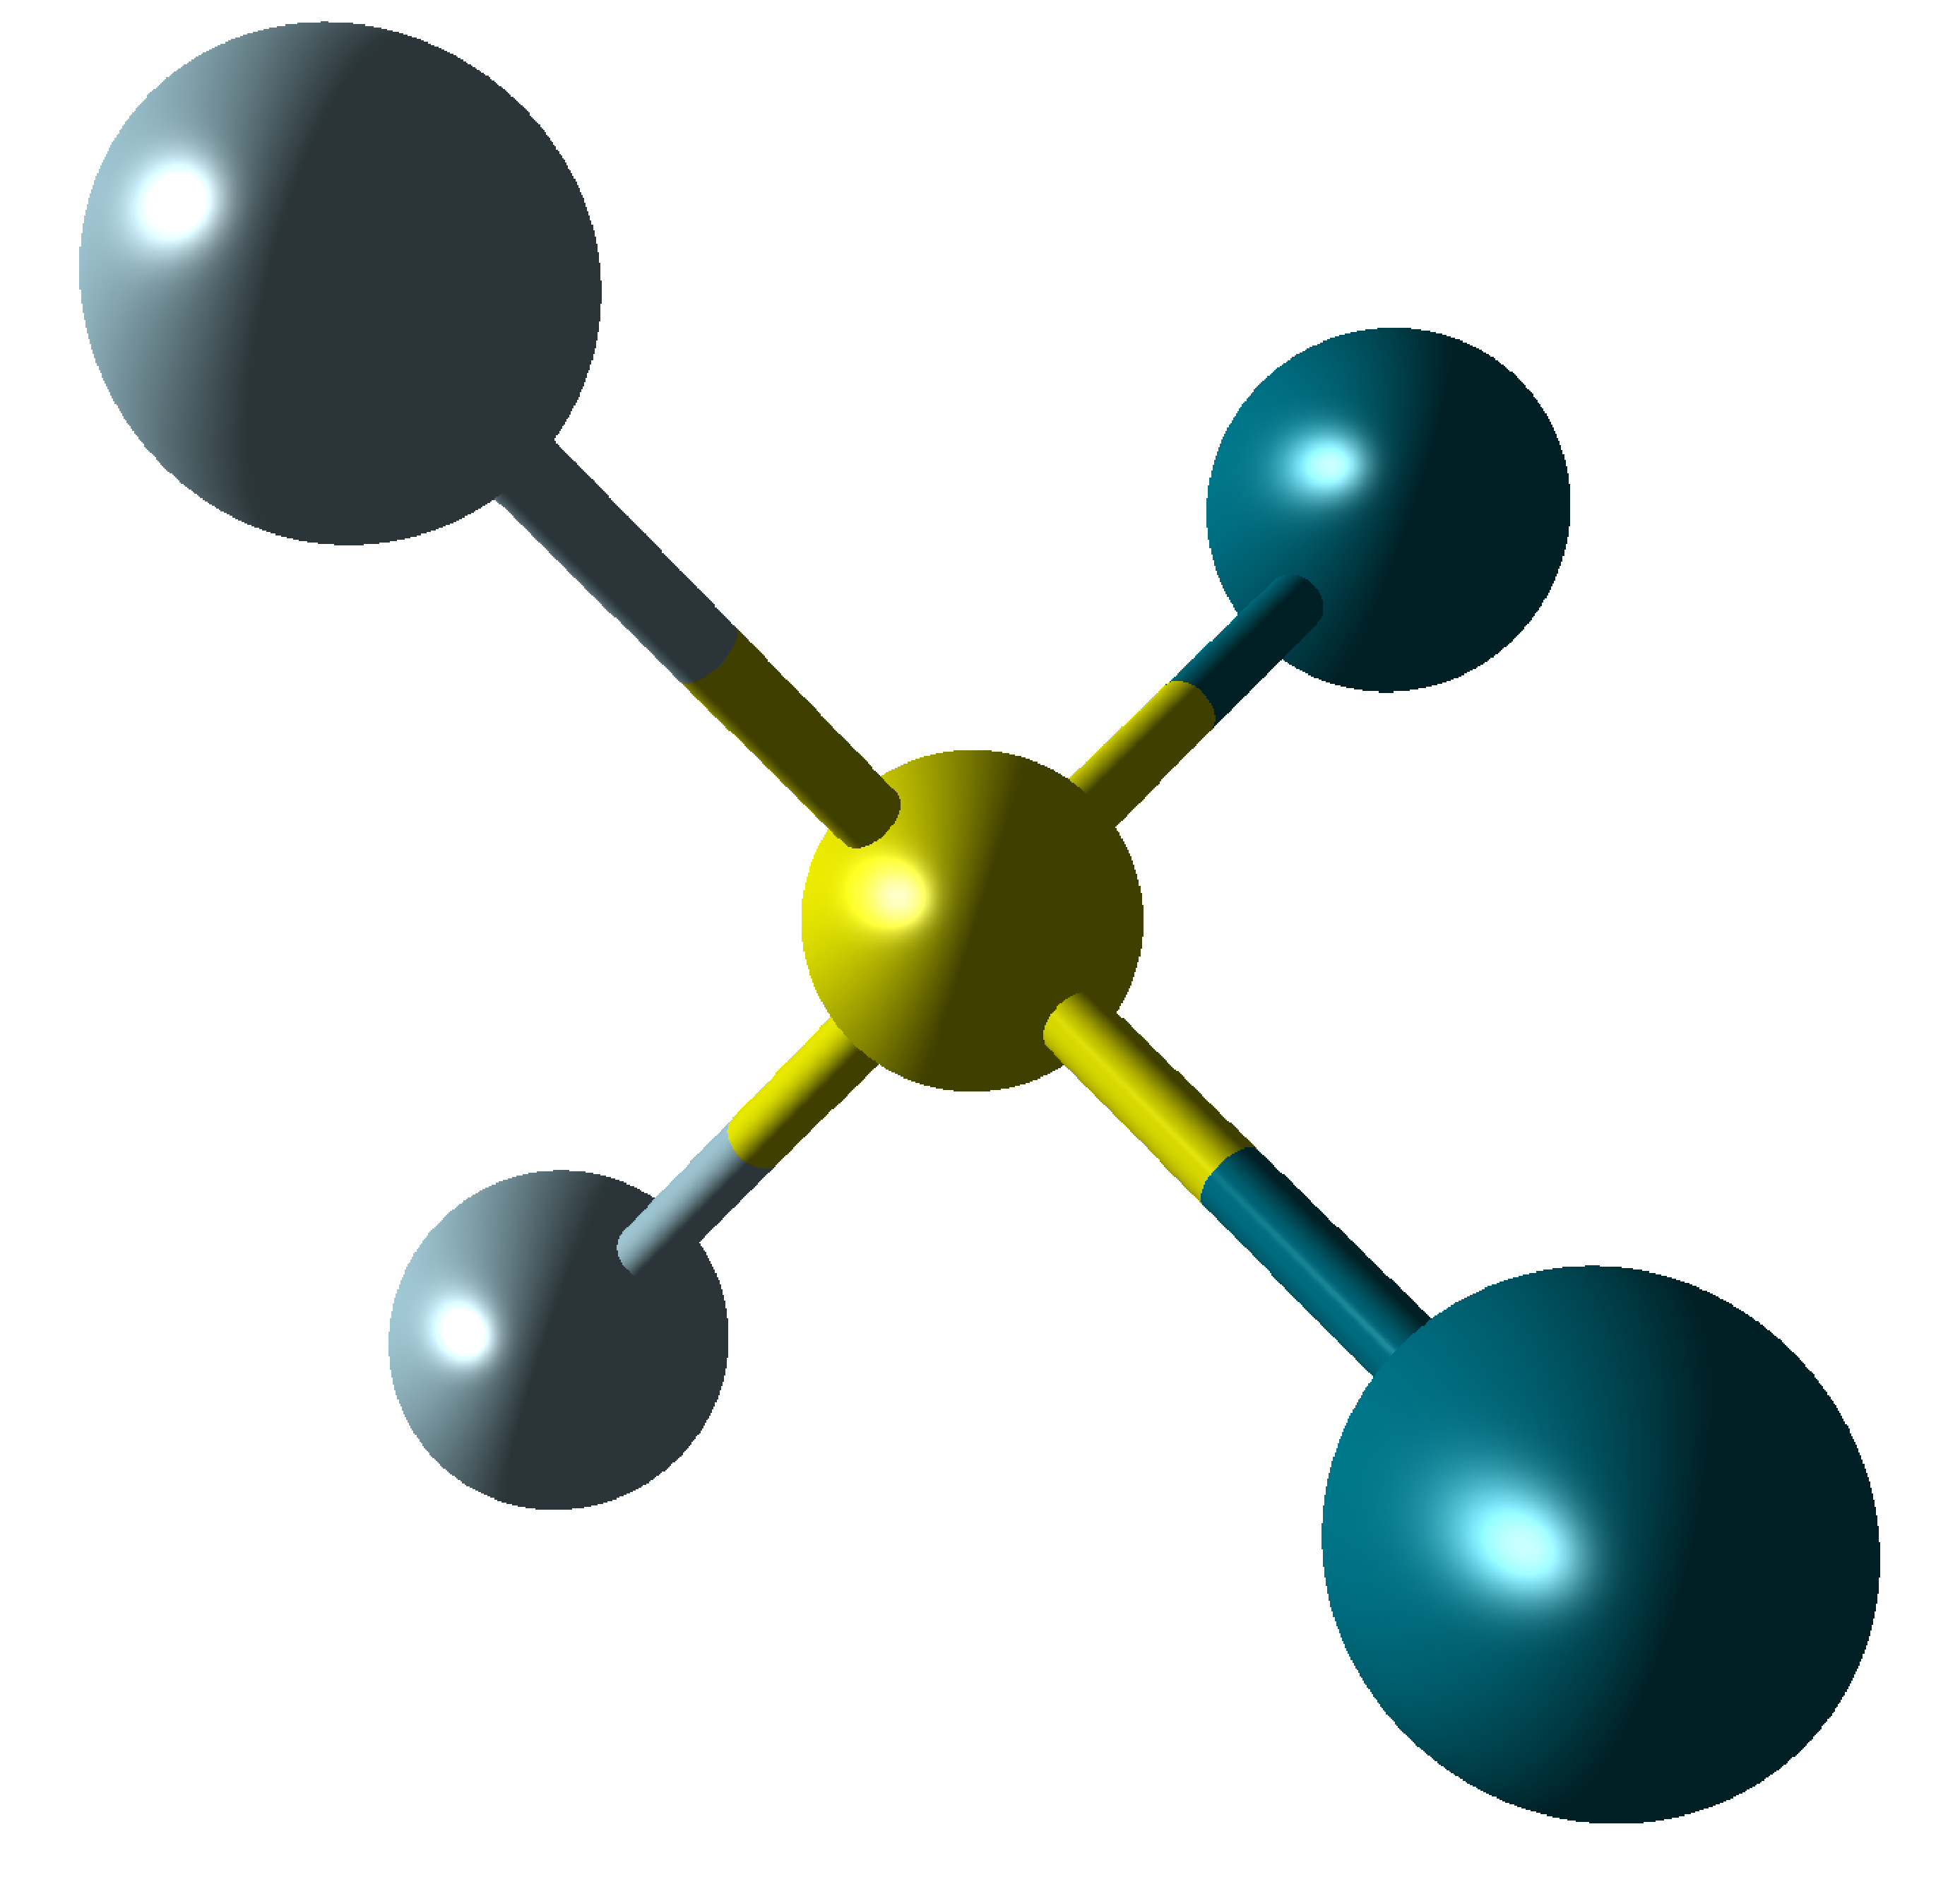
\includegraphics[width=0.17\textwidth]{/media/labfiles/ruco/phd-ssp/phd-codes/symmetry/symmetry0-algaas.pdf}};

\node[anchor = west,xshift=1cm,yshift=0.0cm](a2) at (a1.east){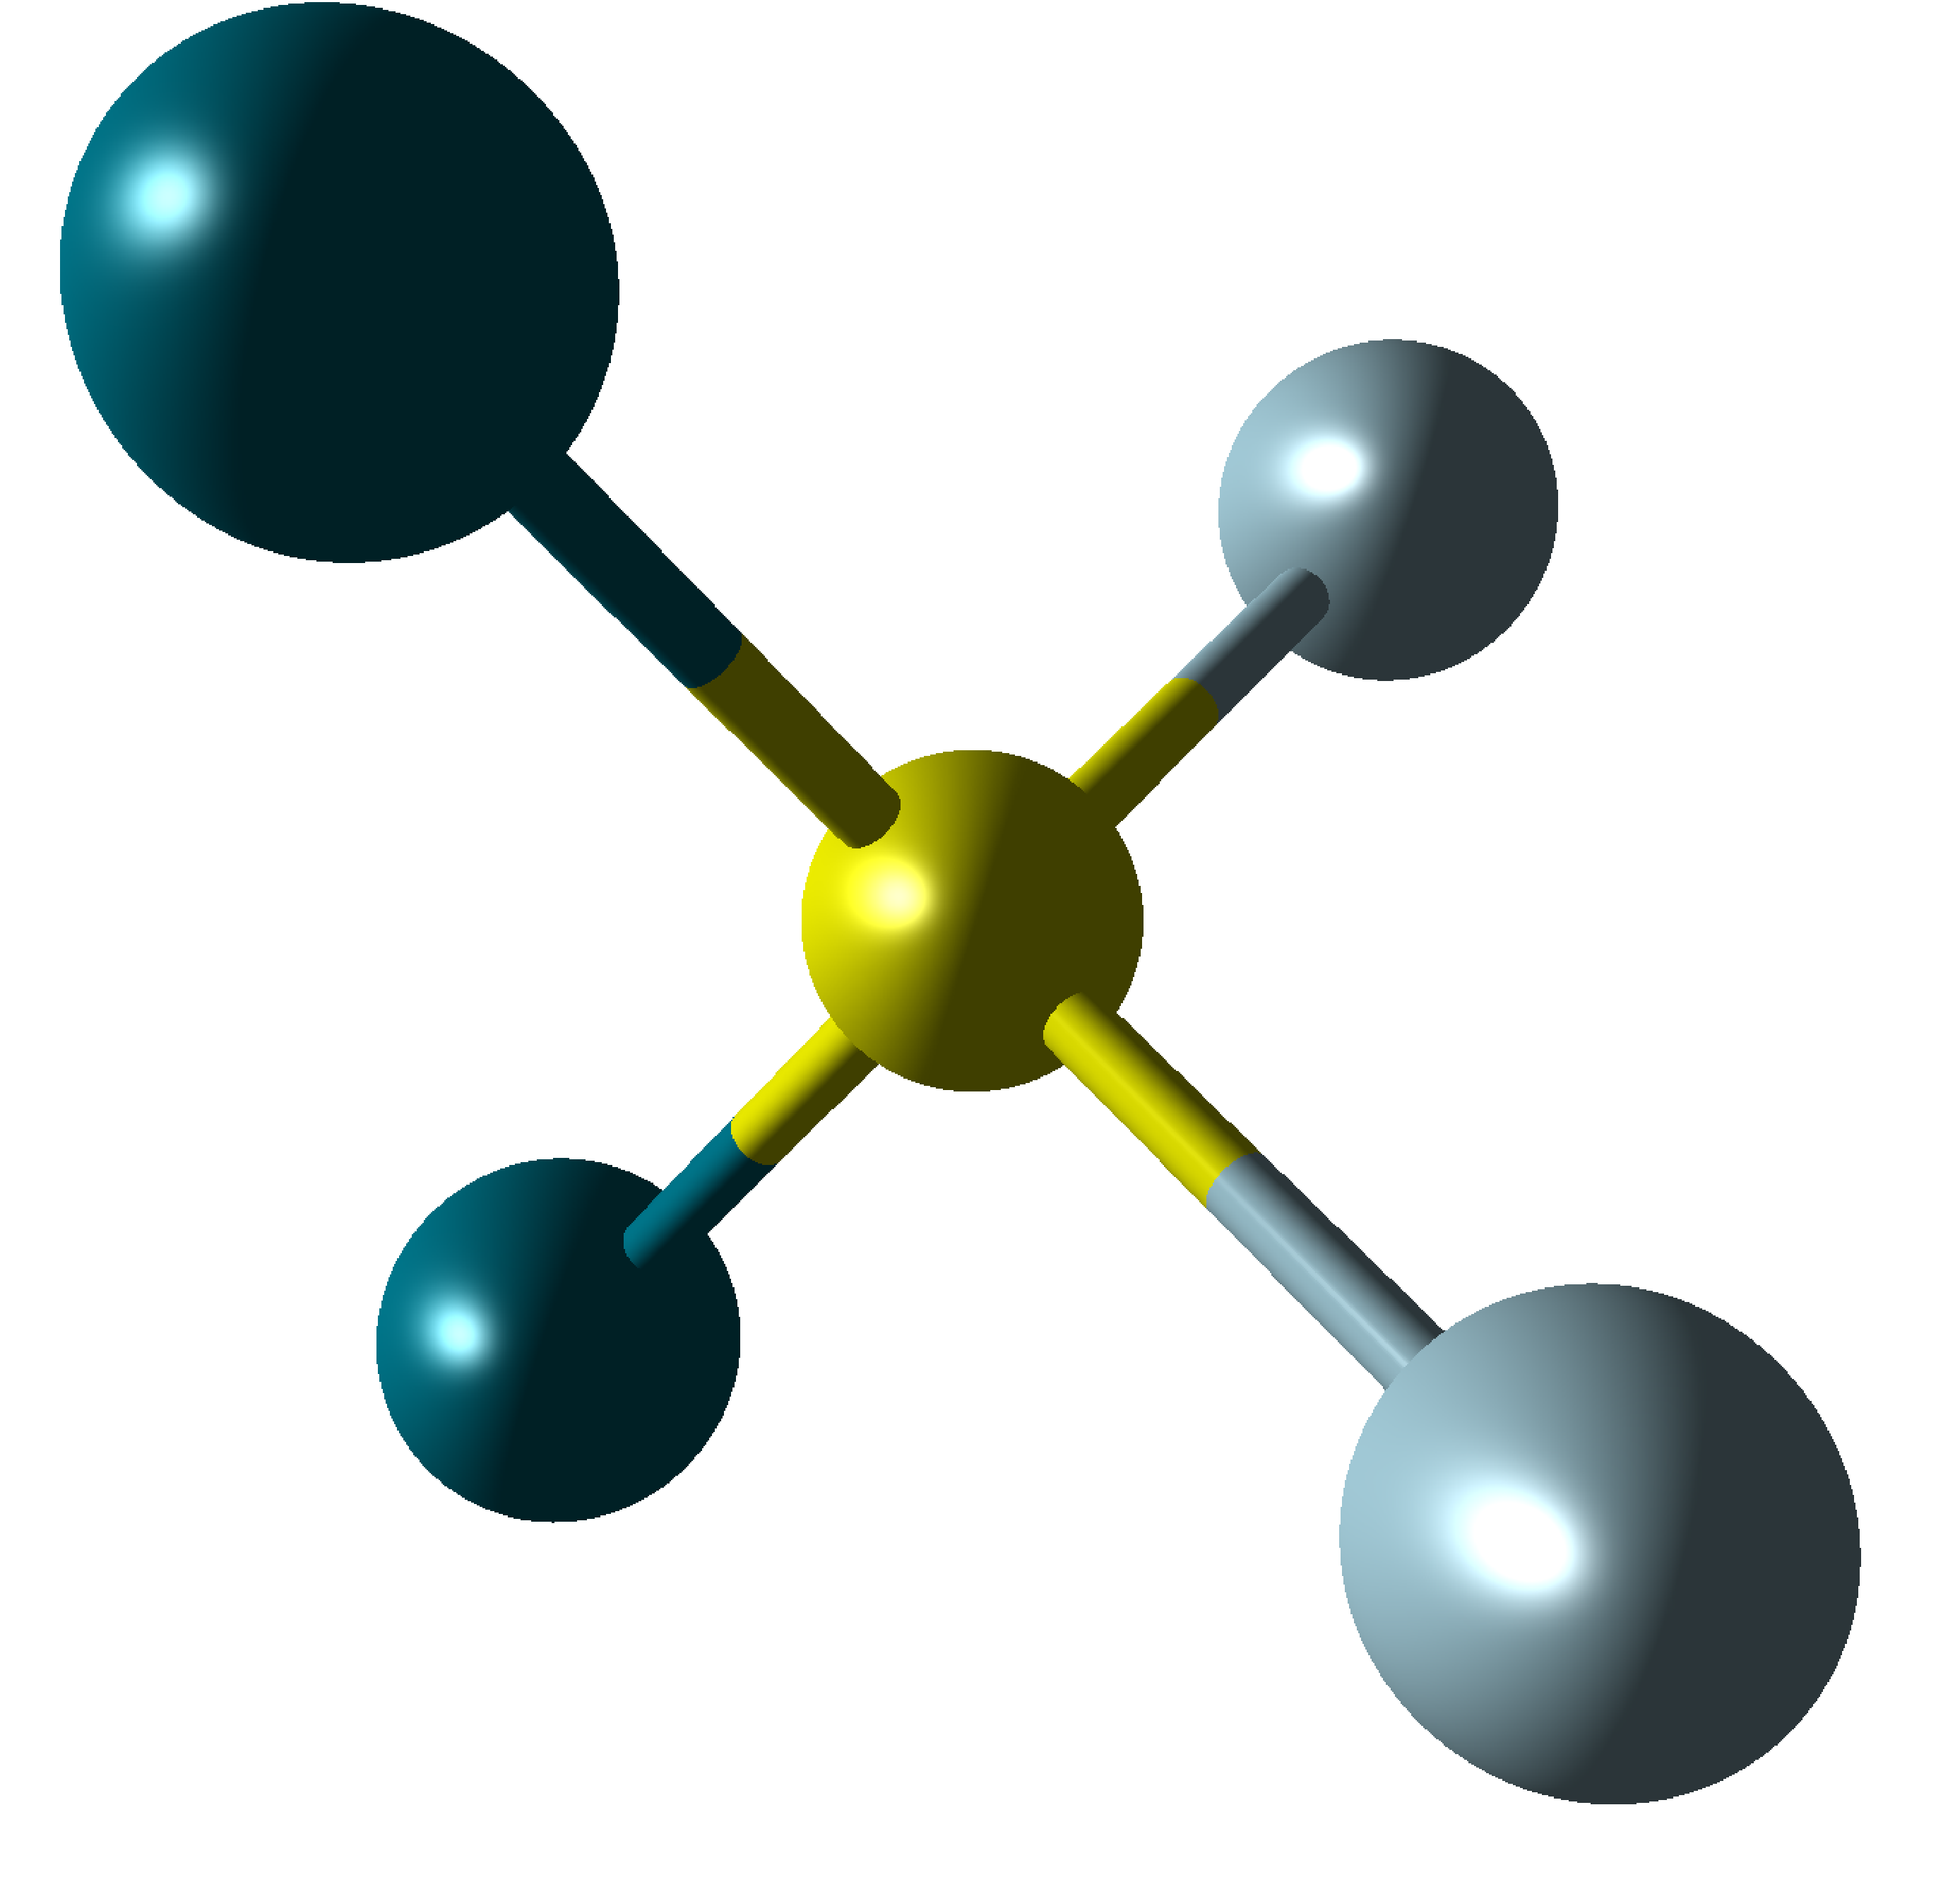
\includegraphics[width=0.17\textwidth]{/media/labfiles/ruco/phd-ssp/phd-codes/symmetry/symmetry1-algaas.pdf}};

\draw[dashed,white] 
	([yshift=2.25cm]current page.west)--
	([yshift=1.75cm]a1.center)--
	([yshift=-2.5cm]a1.center)--
	([yshift=-2.5cm,xshift=3.8cm]a1.center)--
	([yshift=1.75cm]a2.center)--
	([yshift=2.25cm]current page.east);


\draw[fill = Al] ([yshift=2.75cm]current page.west) rectangle ++(1,0.3) 
	node [anchor=west,right,midway,white,xshift=0.5cm] {\(\left(110\right)\)};
\draw[fill = Ga] ([yshift=2.4cm]current page.west) rectangle ++(1,0.3) 
	node [anchor=west,right,midway,white,xshift=0.5cm] {\(\left(1\overline{1}0\right)\)};


\shade [ball color=Ga,white] ([xshift=5mm,yshift=4cm]s1.west) circle (0.2) node[label=right:{\Large\, Ga}] { } ;
\shade [ball color=Al,white] ([xshift=5mm,yshift=3.5cm]s1.west) circle (0.2) node[label=right:{\Large\, Al}] { } ;
\shade [ball color=As,white] ([xshift=5mm,yshift=3cm]s1.west) circle (0.2) node[label=right:{\Large\, As}] { };

\node[white,xshift=-2cm,yshift=2cm]  at (current page.east){Potential edge profile};

\begin{scope}[xshift=1cm,yshift=-6.5cm,rotate around z=0]
	\draw[red, thick,-{Stealth},blue] (0,0,0) -- (3,0,0) 
			node[anchor=west, blue]{$z$};
	\draw[red, thick,-{Stealth}] (0,0,0) -- (0,1,0) 
			node[anchor=south]{$y$};
	\draw[red, thick,-{Stealth},green] (0,0,0) -- (0,0,1) 
			node[anchor=north]{$x$};
\end{scope}
\end{tikzpicture}
	
	

\end{document}